\documentclass[12pt,a4paper]{ctexart}
\usepackage{graphicx}
\usepackage{ctex}
\usepackage{indentfirst}
\graphicspath{{chapter/}{figures/}}
\usepackage{CJK}



\author{周彦百}

\begin{document}

% 封面部分

\begin{titlepage}
	\centering
	
\includegraphics[width=0.2\textwidth]{SchoolLogo}\par
	\vspace{1cm}
	
\includegraphics[width=0.8\textwidth]{SchoolName}\par
	\vspace{0.1cm}
	{\scshape\LARGE Harbin Institute of Technology \par}
	\vspace{1cm}
	{\kaishu\LARGE 材料分析技术学习报告\par}
	\vspace{1.5cm}
	{\huge\bfseries 扫描隧道显微镜\par}
	\vspace{2cm}
	{\fangsong\Large\itshape 周彦百 \par}
	\vfill
	{1708401}\par
	\fangsong{材料科学与工程学院}
	\fangsong{电子封装技术}

	\vfill
% Bottom of the page
	{\large \today\par}
\end{titlepage}

\tableofcontents

\vfill

\section{简介}
扫描隧道显微镜是IBM苏黎世实验室Gerd Binning和Heinrich Rohrer等于1982年发明的一种新型表面测试分析一起。STM具有优异的分辨本领,横向分辨率可达0.1nm,纵向分辨率高达0.01nm。可在真空、大气或液体环境下,在实空间内对样品表面的原子组态进行原位动态观察,并可直接用于观察样品表面发生的物理或化学反应的动态过程及反应中原子的迁移过程等。此外,STM在低温下(4K)可以利用探针尖端精确操纵原子,因此它在纳米科技领域既是重要的测量工具又是加工工具。它的出现被国际科学界公认为是20世纪80年代世界十大科技成就之一。他们两人也因此荣获1986年诺贝尔物理学奖。迄今为止,STM已在物理、化学、材料科学、表面科学、生命科学等领域得到广泛应用。

\section{工作原理}
从经典物理学来说,金属体内存在大量“自由”电子。在绝对零度时,所有自由电子的能量都小于费米能级$E_{F}$,随着温度的升高,一部分电子的能量可以大于费米能级,且温度越高,这部分电子的占比越大。而在金属边界上存在着一个能量高于费米能级的势垒,在金属内的“自由”电子中,只有能量高于这个势垒的电子才能够从金属内部逸出至外部。然而,量子力学则认为,费米子也具有波粒二象性,金属中的电子也不例外,在电子波向金属边界传播时,遇到表面势垒时,部分反射,仍有部分电子穿透金属表面势垒,形成金属表面上的电子云。这种效应称为隧道效应。

两种金属(即电极)靠得很近(通常小于1nm)时,两种金属的电子云将互相渗透,这时假如加上适当的电压,即使两者并未真正接触,也会有电流从一种金属流向另一种金属,这种电流就称为隧道电流。

STM的工作原理简单来说,就是通过制作一具有原子尺度的针尖,工作时就在其与样品间加上一定的电压。当样品与针尖的距离小于一定值时,由于量子隧道效应,样品和针尖间就可产生隧道电流。

在低温低压下,隧道电流$I$可近似的表达为\[I\propto V_{b}exp(-A \Phi^{1/2}d)\]\\
式中:
\begin{quote}
	$V_{b}$——针尖与样品之间所加的偏压;

	$\Phi$——针尖与样品的平均功函数;

	$A$——常数,在真空条件下,$A$近似为1;

	$d$——样品与针尖间的距离。
\end{quote}

由此式可见,隧道电流$I$并非样品表面起伏的简单函数,它表征样品和针尖电子波函数的重叠程度。由该式计算可得,样品与针尖间的距离每减少0.1nm时,隧道电流$I$的强度将增大一个数量级,即隧道电流$I$对样品表面的微观起伏特别敏感。扫描探针一般采用直径小于1mm的细金属丝,被观测样品应具有一定的导电性才可以产生隧道电流。

\section{工作方式}
\subsection{恒电流模式}
利用一套电子反馈线路控制隧道电流$I$,使其保持恒定。再通过计算机系统控制针尖在样品表面扫描,即是使针尖沿x、y两个方向作二维运动。由于要控制隧道电流$I$不变,针尖与样品表面之间的局域高度也会保持不变,因而针尖就会随着样品表面的高低起伏而作相同的起伏运动,高度的信息也就由此反映出来。这就是说,STM得到了样品表面的三维立体信息。这种工作方式获取图象信息全面,显微图象质量高,应用广泛。
\subsection{恒高度模式}
在对样品进行扫描过程中保持针尖的绝对高度不变;于是针尖与样品表面的局域距离将发生变化,隧道电流$I$的大小也随着发生变化;通过计算机记录隧道电流的变化,并转换成图像信号显示出来,即得到了STM显微图像。这种工作方式仅适用于样品表面较平坦、且组成成分单一(如由同一种原子组成)的情形。 从STM的工作原理可以看到:STM工作的特点是利用针尖扫描样品表面,通过隧道电流获取显微图像,而不需要光源和透镜。这正是得名“扫描隧道显微镜”的原因。

\section{应用领域}
\subsection{表面显微表征}
STM由于对表面起伏十分敏感,可用于非常精细的材料表面科学观测、微观表征,对研究和验证材料的结构和性能有着巨大的帮助作用。
\subsection{探伤及修补}
正如前面提到的,STM既是一种测量工具也是一种加工工具。它可以在观察到材料表面的细微损伤和缺陷后,用表面淀积和刻蚀等方法建立或切断连线,以消除缺陷,达到修补的目的,然后还可用STM进行成像以检查修补结果的好坏。
\subsection{移动、刻写样品}
当STM在恒流状态下工作时,突然缩短针尖与样品的间距或在针尖与样品的偏置电压上加一脉冲,针尖下样品表面微区中将会出现毫微米级的坑、丘等结构上的变化。针尖进行刻写操作后一般并未损坏,仍可用它对表面原子进行成像,以实时检验刻写结果的好坏。

移动针尖进行刻写的办法主要有两种:
\begin{enumerate}
	\item 在反馈电路正常工作时,通过调节参考电流或偏置电压的大小来调节针尖与样品间的接触电阻,达到控制针尖移动的目的。当加大参考电流或减小偏压时为保证恒流工作,反馈将控制针尖移向样品,从而减小接触电阻。
	\item 当STM处于隧道状态时,固定反馈线路的输出信号,关闭反馈,然后通过改变控制Z向运动的压电陶瓷上所加电压的大小来改变针尖与样品的间距,这种方法较前者能够更线性地控制隧道结宽度的变化,相对来说是较为理想的办法。
\end{enumerate}

\begin{figure}
	\centering
	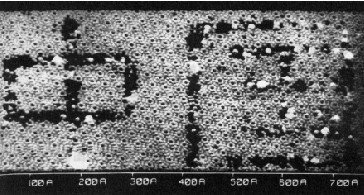
\includegraphics[width=0.8\textwidth]{figures/stm}
	\caption[ZhongGuo]{1993年科学家利用STM在硅原子上写下的“中国”}
	\label{fig:ZhongGuo}
\end{figure}

刻写的结果与针尖的清洁程度有密切关系。已经污染的针尖接触表面后将产生一小坑;未使用过的清洁的针尖接触表面则产生一小丘。清洁针尖在表面上产生小丘的原因是由于它与表面有粘接现象,此时若想使针尖与样品的间距恢复到与表面接触前的情况,针尖必须退回更多,这从另一个角度说明针尖的粘接已使表面产生一凸起部分。针尖的污染将会阻止它对表面的粘接,故使用过的针尖接触表面后将会刻出一个小坑,坑的周围还会有原先在坑内的原子翻出堆成的凸起边缘。

室温下在Au及Ag等金属表面上刻写出的微细结构在室温下总是不稳定的,由于金属原子的扩散,这些结构最多在几小时内就会模糊以至消失。

在其他材料如Si(110)、Si(100)等表面上运用STM刻出稳定的结构却是可能的。刻写时,针尖向样品移进2nm时,小坑深(从边缘算起)0.7nm。在室温条件下及超高真空中,这些图形具有高稳定性,经很长时间后亦不发生变化。

\section{结语}
可以看到,扫描隧道显微镜是利用尖端科学成果从而实现人们对材料、物质的深入认知的一门新兴的表面显微分析测试技术。其技术尚有很大的发展空间和前景,学会使用它,并利用它鲜明的图案带给我们的更深一层的理解力去理解世界,是我们最终追求的目标。

\end{document}
